\chapter{DAH Checkpoints}
\label{sec:checkpoints}
\vspace*{-0.99cm}
{\bf Important note}: Please consult the DAH manual to familiarise yourself with the equipment, including the Raspberry Pi, LEDs, temperature sensors, ADCs, DACs, I/O, switches, breadboard and connectors.
The manual contains detailed instructions on how to operate the Raspberry Pi.
To copy python code snippets (see below) into your python scripts, download these files from github, see \url{https://github.com/fmuheim/DAH}.
Data sheets for all electronic elements are available from Dropbox, see: \url{https://www.dropbox.com/sh/gfnisnh4ntnum1d/AAAWtNL_AhcpR8PZ_QmqZpsja?n=112609310}.  

\section{Checkpoint 1: LEDs and Switches}

\begin{enumerate}
\item [1.1.] Control an LED with the Raspberry Pi by completing the following steps.
Connect the Raspberry Pi to a breadboard using the adapter.
On the breadboard, connect GPIO~24 to an LED with a 1~kOhm resistor in series to ground: this is a ``positive logic'' or ``active high'' circuit, as descibed in the lab manual.

\vspace*{-3mm}
\begin{center}                                        
{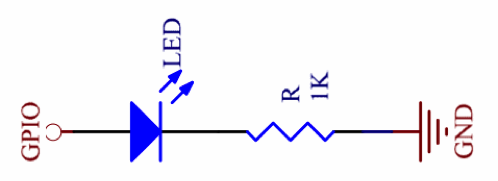
\includegraphics[width=10cm]{figs/ActiveHighLED}}
\end{center}

\newpage
Using this code template, import the GPIO library and turn the LED on and off.
\lstinputlisting{../scripts/checkpoint_1a.py}

Repeat the exercise with negative logic (active low) by connecting the LED with a 1~kOhm resistor in series to 3.3~V.
Draw a schematic diagram for this circuit like the example above.
 

\item [1.2.] Modify the first python script to blink the LED continuously.
You can do this by adding a while loop. \\

\lstinputlisting{../scripts/checkpoint_1b.py}

Since this code will keep running forever, you'll need to press CTRL+C to stop it.
 

\item [1.3.] Using positive logic (active high) connect a push-button switch between 3.3V and GPIO23 and, with a 1~kOhm resistor in series, to ground.
See the diagram in your lab manual for more information.
Modify your python script to toggle the LED state every time the push button switch is pushed. \\

\lstinputlisting{../scripts/checkpoint_1c.py}

\end{enumerate}

{\bf This checkpoint is not assessed.}


\newpage
\section{Checkpoint 2: ADC, DAC and SPI BUS}

Most experimental observables are continuous: their values can vary by arbitrarily small amounts.
However, we record measurements as discrete values: a number with some range of uncertainty.
Creating a numerical (digital) measurement from a continuous (analogue) signal is called digitisation, and is performed by an Analogue to Digital Converter (ADC).
The digital information can then be analysed with a computer.

In this checkpoint we will use an ADC to read information from a light sensor into the Raspberry Pi.
We will also perform the opposite task, varying the brightness of an LED by converting a numerical output from the Raspberry Pi into the corresponding voltage level using a Digital to Analogue Converter (DAC).

\vspace*{-0.5cm}
\begin{enumerate}

\item [2.1.] Connect an ADC MCP3208 chip to the Raspberry Pi using the SPI Interface.
Make sure that all required connections between the MCP3208 and the Raspberry Pi are made (see lab manual).
Use a multimeter to check that power (VDD) and ground (AGND and DGND) are correctly connected.

Connect a Light Dependent Resistor (LDR) and a 4.7~k$\Omega$ resistor as a voltage divider between 3.3 and 0~V, using an ADC input channel to measure the voltage in the middle.
Use python to read the voltages of all eight ADC channels.
Try reading a specific ADC channel, and experiment with all the other methods given below.
You are encouraged to consult the following webpage \url{http://webiopi.trouch.com/}($\rightarrow$ Tutorials $\rightarrow$ Using Devices $\rightarrow$ Analog).

\lstinputlisting{../scripts/checkpoint_2a.py}
\vspace*{-0.5cm}

\newpage
\item [2.2.] Leave the ADC in place, but also connect the DAC MCP4922 chip to the Raspberry Pi.
Make sure that all required connections between the MCP4922 and the Raspberry Pi are made (see lab manual).
Use a multimeter to check that power (VDD) and ground (AVSS) are correctly connected.

Use python to set a value --- e.g. 1.3~V --- to output VOUTA of the DAC.
Measure this voltage with a multimeter. \\

\lstinputlisting{../scripts/checkpoint_2b.py}
%\vspace*{-0.5cm}

\item [2.3.] Connect one output of the DAC to an LED.
Write a python script that varies the brightness of the LED by setting a series of different values for the output voltage of the DAC.
Now arrange the circuit so that the LED is next to the LDR, and the change in brightness can be measured.
The laboratory is quite bright relative to an LED, so you might need to cover the breadboard to show a convincing change.
Modify your script to read the ADC input each time you set the DAC output.
Write the DAC setting and measured ADC values at each step to an output file with comments such that the content of the file will explain your work.

\end{enumerate}

{\bf NB:} Do not dismantle your circuit after this checkpoint!
You can re-use most of it for Checkpoint~3.

\newpage
{\bf Assessment tasks: submit in Learn}

\begin{itemize}

\item Submit a document with the following information:
\begin{enumerate}
\item Explain what all connections to the ADC chip are for (do not simply copy information from the datasheet --- explain the practical purpose of these connections).
\item Explain the meaning of the return values of each Python method for the ADC.
\item What is the primary (most fundamental) ADC output and how is the final voltage output calculated from this?
\item Explain how the ADC readings change when you cover the LDR with your hand --- you may need to provide a circuit diagram.
\item Explain what all the connections to the DAC chip are for.
\end{enumerate}
\hfill {\bf[5~marks]}

\item Submit a photograph of your multimeter measuring (approximately) 1.3~V output from the DAC.
\hfill {\bf[2~marks]}

\item Submit your code that controls the LED brightness using the DAC, and monitors the effect on the LDR using the ADC.
\hfill {\bf[2~marks]}

\item Submit your output file.
\hfill {\bf[1~mark]}

\end{itemize}


\newpage
\section{Checkpoint 3: Sampling Analogue Signals}

\begin{enumerate}

\item [3.1.] Connect an ADC chip (MCP3208) to the Raspberry Pi, as in Checkpoint 2 (or re-use your existing circuit).

Use the bench-top signal generator to produce a repetitive signal, e.g. a sinusoidal waveform.
Display the output on the oscilloscope.
Set the amplitude of the signal such that the waveform can be read by the ADC chip, which can sample between 0~V and VREF = 3.3~V. Set the frequency to 10~Hz.

Connect the output of the signal generator to an ADC input channel.
Don't connect a signal with a voltage outside the range of the ADC chip: this could destroy it (and the Raspberry Pi)!
Use python to read a few measurements from the ADC, and make sure they behave as you expect.

%\hfill [1 marks]\\

\item [3.2.] Measure the waveform produced by the signal generator by writing a python script that records 100 ADC samples and displays these on a graph of voltage vs time.
Calculate the approximate time between samples by measuring the start and end times of your sampling and dividing the difference by 100.
You can use the pylab interface for plotting graphs --- example files are available on GitHub.
Always label plots correctly with title and axes and save these to a file (pdf format).

%\hfill [2 marks] \\

%\item [3.3.] Calibrate the voltage scale of the ADC output with respect to the voltage scale displayed on the oscilloscope by using a square waveform that closely matches the ADC input range.   First connect the signal from the signal generator to the oscilloscope. Read the input voltage for the high and low sections of the square waveform off the oscilloscope screen. For this use the trigger threshold dial to determine these voltage levels as precisely as possible. Then connect the signal to an ADC input channel. Write a python script that takes 100 ADC samples and writes these into a file, then expand the script to determine the average ADC voltages for the high and low sections of the square waveform and record the results. Reduce the amplitude of the input waveform by a factor of two and repeat above procedure. Plot the four calibration measurements, i.e. the measured ADC voltages (from the two sets of measurements of the  high and low sections) versus the four input voltages (measured with the oscilloscope) on a graph and comment.

%\hfill [2 marks] \\

\item [3.3.] Given the time that you calculated elapses between ADC samples, what is the highest input signal frequency that you can expect to measure correctly?
(You may wish to research signal sampling a little before jumping to your answer...)
Test input signals at a range of different frequencies to see if the results are as you expect.

%\item[3.4.]	What is the maximum signal frequency with which you can properly record a given repetitive signal?   First, consider which would be the best waveform for this investigation. What is the sampling frequency? Explain what happens when a signal is undersampled. Make a plot with a waveform that is undersampled.   

%\hfill [2 marks] \\

%\item [3.5.] Connect a DAC chip (MCP4922) to the Raspberry Pi, as in Checkpoint 2.  Using a python script, generate a sinusoidal waveform on the DAC output and plot the waveform to a graph.

%Use the ADC chip (MCP3208) to digitise the waveform generated by the DAC. Write a python script that takes 100 DAC samples and 100 ADC measurements and plot these on the same graph. Take into account the limitations encountered in 3.4.                                                          
 
%\hfill [3 marks] 

\end{enumerate}

{\bf Assessment tasks: submit in Learn}

\begin{itemize}

\item Submit your code for measuring the signal generator output with your ADC.
\hfill {\bf[2~marks]}

\item Submit a plot showing 100 sampled values from a 10~Hz sinusoidal signal.
\hfill {\bf[1~mark]}

\item Submit a document with the following information:
\begin{enumerate}
\item What time did you calculate elapsed between samples?
\item What did you calculate was the highest signal frequency you can measure correctly (and why)? Provide a plot showing your sampling of an input waveform at this frequency.
\item Explain what happens when a waveform is undersampled, and provide a plot that shows what you describe.
\end{enumerate}
\hfill {\bf[3~marks]}

\end{itemize}

\newpage
\section{Checkpoint 4: Input/Output and I2C BUS}

\begin{enumerate}


\item [4.1.] Input/Output (I/O) Expander chips enable the user to connect many devices that have the same or similar functions.
With the Raspberry Pi this can be achieved using the I2C bus.
Connect the PCF8574AN chip  (I2C BUS Expander) to the Raspberry Pi.
Make sure that all required connections between the PCF8574AN chip and the Raspberry Pi are made, as shown in the lab manual.

Using negative logic connect an LED to output P0 of the PCF8574AN Expander chip. 
Write a python script to blink the LED, similar to what you did in Checkpoint 1.

You may consult the \webiopi webpage \url{http://webiopi.trouch.com/} ($\rightarrow$ Tutorials $\rightarrow$ Using Devices $\rightarrow$ Digital) to find information on the GPIO expander chip.

{\bf NB:} The GPIO library used here is different to that used in Checkpoint 1.
The RPi.GPIO definitions are not compatible with the \webiopi I/O expander commands. \\

\lstinputlisting{../scripts/checkpoint_4a.py}

\item [4.2.] Connect an additional 3 LEDs to outputs P1, P2 and P3 of the PCF8574AN Expander chip.
Write a python script which turns the LEDs on and off in a cycle of defined patterns, using the portWrite(value) method to control all four LEDs at the same time.
Experiment with portWrite and make sure you understand how the value you pass to it affects the LEDs.

%\newpage
%\item [4.3.] Consult the webpage \url{http://webiopi.trouch.com/} ($\rightarrow$ Tutorials $\rightarrow$ Using Devices $\rightarrow$ Digital) for the GPIO Expander. Use the portWrite(value) method to manipulate all four LEDs at the same time.  Connect a push button switch to pin P4 of the expander chip. Write a python script such that an LED pattern toggles every time the button is pushed.\\

%\lstinputlisting{../scripts/checkpoint_4b.py}
%\hfill [3 marks]\\

\end{enumerate}

\newpage
{\bf Assessment tasks: submit in Learn}

\begin{itemize}

\item Submit a document with the following information:
\begin{enumerate}
\item Explain the purpose of the SDA, SCL and A0, A1, A2 connections to the PCF8574AN chip.
\item If you were to connect the A0 pin to +3.3~V instead of ground, how would you modify your code?
\item Why is it necessary to connect the LED to the chip using negative logic, rather than positive (consider the direction of current)?
\end{enumerate}
\hfill {\bf[3~marks]}

\item Submit your code where you use the portWrite command to display multiple different patterns with four LEDs.
Ensure that the code comments explain how your inputs to portWrite create a particular pattern.
\hfill {\bf[2~marks]}

\item Submit photos (or video if possible) of the LEDs changing as your code runs.
\hfill {\bf[1~mark]}

\end{itemize}


\newpage
\section{Checkpoint 5: Temperature Sensors}

\begin{enumerate}

\item [5.1.] We will be using DS18B20 temperature sensors for this checkpoint.
Take a look at the datasheet here: \url{http://www.adafruit.com/datasheets/DS18B20.pdf} or download it from the DAH Dropbox.

Connect a DS182B0 temperature sensor to your Raspberry Pi (look at the flat front of the sensor to get it the right way around):
\begin{center}
    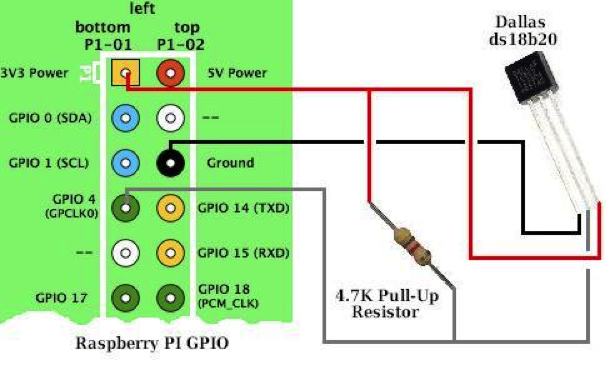
\includegraphics[width=14cm]{figs/DS182B0}
\end{center}

%What is the interface between the DS18B20 temperature sensor and the Raspberry Pi? Explain how it works. 

%Install the drivers for the sensor on the Raspberry Pi with the following commands:
%    pi@Demonstrator-pi ~ $   sudo modprobe w1-gpio
%    pi@Demonstrator-pi ~ $   sudo modprobe w1-therm
%
%Note that you will need to do this again if you restart the Raspberry Pi.

Locate the sensor output by finding the file that has the serial number of your sensor:
\begin{verbatim} 
    studentnn@dahpimm ~ $  cd /sys/bus/w1/devices 
    studentnn@dahpimm /sys/bus/w1/devices $ ls 
    10-00080265b6d6 w1_bus_master1 
\end{verbatim}
Note that your temperature sensor won't be called 10-00080265b6d6, this is just an example.

Now read the sensor output, i.e. the raw temperature measurement:
\begin{verbatim}
    studentnn@dahpimm /sys/bus/w1/devices ~ $ cd 10-00080265b6d6
    studentnn@dahpimm /sys/bus/w1/devices/10-00080265b6d6 $ cat w1_slave 
    30 00 4b 46 ff ff 0d 10 29 : crc=29 YES 
    30 00 4b 46 ff ff 0d 10 29 t=23937 
\end{verbatim}
This should be interpreted as $23.937^{\circ}$C.

\newpage
WebIOPi provides a simple way to access the temperature sensor data in python.
\lstinputlisting{../scripts/checkpoint_5a.py}

Test this method yourself, with a loop taking temperature measurements and displaying them on the screen.

%\hfill [2 marks]


\item[5.2.] Measure temperature with the DS18B20 sensor versus time.
Choose a sensible time interval, and note that taking a single temperature measurement is quite slow.
Write a python script to make a graph of 50 temperature measurements versus time.
Always label plots correctly with title and axes and save these to a file.
 
%As a second step the graph should update itself as each temperature measurement is made.
%Write a python script for this purpose.
%Once this is working, play with it by touching the temperature sensor with your fingers.
%Describe what is happening and sketch it in your lab book.

%The following code example shows how to display a plot that updates regularly: \\
%\lstinputlisting{../scripts/checkpoint_5b.py}
%\hfill [3 marks]



\item[5.3.]	Add another temperature sensor to your circuit by connecting it in parallel with the existing one. 
You don't need to make separate connections to the Raspberry Pi: your new sensor can sit in the same breadboard tracks as the existing one (just make sure that you connect it the right way around).

Find its serial number in the w1/devices folder like before.
Now ensure that you can read out your two temperature sensors simultaneously in python.

%You can test this by running python in interactive mode first. 
%Note that your temperature sensors will have different serial numbers.
%
%\begin{verbatim}
%    studentnn@dahpimm  ~ $ python3
%\end{verbatim}
\lstinputlisting{../scripts/checkpoint_5c.py}
%
%What is the smallest change in temperature that a sensor can report? Explain this with reference to the datasheet, and how the temperature information is encoded.
%
%Investigate the accuracy of the sensor readings by looking at the stability of the measurement with time, and by comparing the outputs of your two sensors. You can probably assume that the ambient temperature in the lab is constant, but shielding your sensors from breezes may help.

%Modify your graphing code from part 5.2 to make histograms of the temperature measurements of the two sensors. 

%You can use the pylab histogram command:\\
%\lstinputlisting{../scripts/checkpoint_5d.py}
%Make also a graph of the difference between the temperature of the two sensors. Determine the RMS value of a set of temperature difference measurements between the two sensors. Explain your results. Are these consistent with the datasheet?

%\hfill [3 marks]

Modify your graphing code from part 5.2 to display data from both temperature sensors on a single graph.


\end{enumerate}

\newpage
{\bf Assessment tasks: submit in Learn}

\begin{itemize}

\item Submit a document with the following information:
\begin{enumerate}
\item What is the interface between the DS18B20 temperature sensor and the Raspberry Pi?
Explain how it works.
\item What is the smallest change in temperature that a single sensor can report?
Explain this with reference to the temperature data encoding described on the sensor datasheet.
\item How do your two temperature sensors' readings compare with each other?
Is this what you would expect from the datasheet?
\end{enumerate}
\hfill {\bf[3~marks]}

\item Submit a plot showing the temperature variation when you touch a sensor with your finger, and then release it.
Annotate the plot, or provide a caption, to explain the shape of the temperature trend line.
\hfill {\bf[1~mark]}

\item Submit your code for plotting measurements from two temperature sensors on the same graph.
\hfill {\bf[2~marks]}

\end{itemize}
